\documentclass[letter]{beamer}
%removed: handout (ignores "animations")

\usepackage[utf8]{inputenc}
\usepackage{graphicx}
\usepackage{minted}

\usetheme{AnnArbor}
%\usetheme{CambridgeUS}
\usecolortheme{beaver}

\title[IIC2333] % (optional, only for long titles)
{05 - Modelos de Redes}
\subtitle{IIC2333 - Sistemas Operativos y Redes}
\author[C.Ruz] % (optional, for multiple authors)
{Cristian Ruz -- {\tt cruz@ing.puc.cl}\footnote{Material preparado con aporte del profesor Carlos Buil Aranda} }
\institute[PUC] % (optional)
{
  Departamento de Ciencia de la Computación\\
  Pontificia Universidad Católica de Chile
}
\date[2/2015] % (optional)
{Semestre 2-2015}
\subject{Informatik}

\AtBeginSection[]
{
  \begin{frame}
    \frametitle{Contenidos}
    \tableofcontents[currentsection]
  \end{frame}
}

\begin{document}

%---------------------------------------------------------------------
\frame{\titlepage}

%---------------------------------------------------------------------
\begin{frame}
\frametitle{Contenidos}
%\tableofcontents[currentsection]
\tableofcontents
\end{frame}


%---------------------------------------------------------------------
\section{Introducción}

\subsection{Motivación}

\begin{frame}
  \frametitle{Los caminos de las redes}

  ¿Qué pasa cuando hacemos {\em click} en un enlace del {\em browser}?
  
  \begin{itemize}
    \item<2-> Evento de {\em hardware}
    \item<2-> Interrupción para el Sistema Operativo
    \item<2-> Evento entregado a proceso {\em browser}
    \item<3-> Proceso {\em browser} interpreta el evento
    \item<3-> Proceso {\em browser} descubre que necesita obtener un {\em recurso}
    \item<3-> Recurso es solicitado mediante {\em syscall} al Sistema Operativo
  \end{itemize}

  \onslide<4->{¿Y después?}

\end{frame}
%---------------------------------------------------------------------
\begin{frame}
  \frametitle{Infraestructura de Redes}

  \begin{block}{Objetivo}
    Permitir que un proceso se {\bf comunique} con otro
  \end{block}
  
  \begin{itemize}
    \item ¿Dónde se encuentra el otro proceso?
      \begin{itemize}
        \item Si se encuentra en la misma máquina: {\em pipe}, {\em shared memory}
        \item Si no, S.O. debe utilizar el sistema de Entrada/Salida
      \end{itemize}
    \item ¿Qué medio utilizar para el envío? (Cable, aire, \ldots)
      \begin{itemize}
        \item ¿Cómo expresar un mensaje en ese medio? Problema Físico
      \end{itemize}
    \item ¿Cómo se envía información por un medio de red?
      \begin{itemize}
        \item ¿Cómo se transmite el mensaje? ¿Se manda completo?
      \end{itemize}
    \item ¿A quién se le transmite el mensaje?
      \begin{itemize}
        \item ¿Hay sólo un receptor? ¿lo estoy ``gritando'' a todos?
      \end{itemize}
    \item ¿Cómo se encuentra el destinatario?
      \begin{itemize}
        \item Destinatario debe tener una dirección ``única''
        \item ¿Cómo ``encaminar'' el mensaje?
      \end{itemize}
    \item El destinatario, ¿está dispuesto a recibir el mensaje?
      \begin{itemize}
        \item Comunicación debe seguir un orden: {\em protocolo}
      \end{itemize}
  \end{itemize}

\end{frame}

%---------------------------------------------------------------------
\subsection{Aplicaciones de Redes}

\begin{frame}
  \frametitle{¿Para qué hacer que dos procesos se comuniquen?}

  Más que nunca, aplicaciones para comunicación de procesos {\em remotos}
  \begin{itemize}
    \item {\bf Compartir recursos}. Muy tradicional.
      \begin{itemize}
        \item Recursos: impresoras, discos, archivos, ciclos de CPU
        \item Acceso a recursos {\em escasos} que no se encuentran {\em geográficamente} cerca
        \item Modelo {\bf cliente-servidor}
      \end{itemize}
  \end{itemize}
  
  \begin{center}
    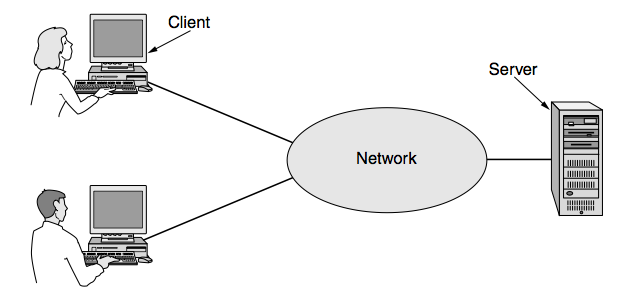
\includegraphics[width=8cm]{figs/05-clientserver.png}
  \end{center}
  
  \begin{itemize}
    \item WWW, Email, Telefonía IP, documentos compartidos, \ldots
  \end{itemize}

\end{frame}

%---------------------------------------------------------------------
\begin{frame}
  \frametitle{¿Para qué hacer que dos procesos se comuniquen?}

  \begin{quote}
    There is no reason for any individual to have a computer in his home
    \begin{flushright}Ken Olsen, president of DEC, 1977\end{flushright}
  \end{quote}

  \begin{itemize}
    \item Múltiples puntos de acceso de información. Ser cliente {\bf Y} servidor
    \item Modelo {\bf peer-to-peer}
  \end{itemize}
  \begin{center}
    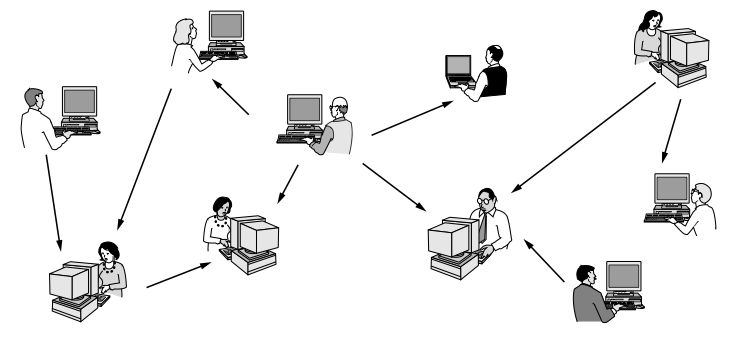
\includegraphics[width=5cm]{figs/05-peertopeer.png}
  \end{center}
  \begin{itemize}
    \item Recursos decentralizados: BitTorrent
    \item Grafos de comunicación: redes sociales
    \item Mensajería instantánea
    \item {\em Streaming}
  \end{itemize}

\end{frame}
%---------------------------------------------------------------------
\begin{frame}
  \frametitle{¿Para qué hacer que dos procesos se comuniquen?}

  Comunicación móvil
  \begin{itemize}
    \item<2-> Conexiones esporádicas: hotspots inalámbricos
    \item<3-> Comunicación por cercanía: RFID
    \item<4-> Mensajería móvil: SMS
    \item<5-> Sistema de ubicación geográfica: GPS
    \item<6-> Redes de sensores
    \item<7-> Dispositivos {\em wearable}
  \end{itemize}

\end{frame}

%---------------------------------------------------------------------
\begin{frame}
  \frametitle{Riesgos y amenazas}

  \begin{itemize}
    \item ¿Cómo viaja la información?
      \begin{itemize}
        \item ¿Está bien que cualquier persona puede verla?
        \item {\em Cookies} y {\em profiling} de usuarios
      \end{itemize}
    \item Confiabilidad de la información
      \begin{itemize}
        \item Ataques de ingeniería social: {\em phishing}
        \item Protocolos de seguridad
      \end{itemize}
    \item Autentificación de clientes
      \begin{itemize}
        \item ¿Humano o {\em bot}?: CAPTCHA
        \item Transmisión de información sensible
      \end{itemize}
    \item Amenazas al desempeño
      \begin{itemize}
        \item Denegación de servicio distribuida (DDOS)
        \item {\em Botnets}
      \end{itemize}
    \item Aspectos legales
      \begin{itemize}
        \item Leyes de neutralidad
        \item Leyes de ``protección'' de {\em copyright}
      \end{itemize}
  \end{itemize}
  
\end{frame}
%---------------------------------------------------------------------
\section{Conceptos de {\em Hardware}}

\subsection{Definiciones}

\begin{frame}
  \frametitle{Elementos de red}

  \begin{center}
    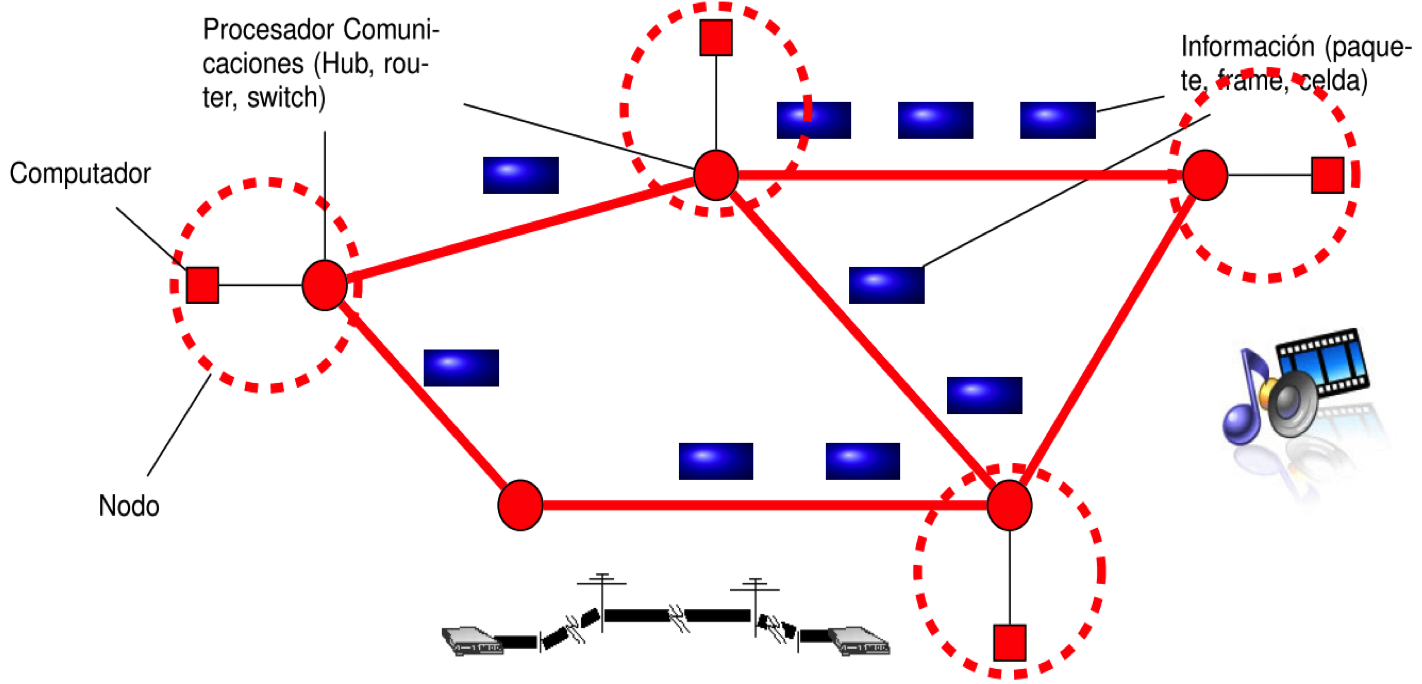
\includegraphics[width=10cm]{figs/05-definiciones.png}
  \end{center}

\end{frame}


%---------------------------------------------------------------------
\subsection{Redes por tecnología de transmisión} 

\begin{frame}
  \frametitle{Primeros conceptos de red}
  \framesubtitle{Tecnología de transmisión}

  {\bf ¿A quién se transmite la información?}
  \begin{itemize}
    \item {\bf Broadcast}: todos la reciben
    \item {\bf Punto a punto}: solo emisor y destinatario
  \end{itemize}
  
  \begin{center}
    
\includegraphics[width=2cm]{figs/05-wally1.png}
    
\includegraphics[width=7cm]{figs/05-wally2.png}
  \end{center}
    

\end{frame}

%---------------------------------------------------------------------
\begin{frame}
  \frametitle{Tecnología de transmisión}
  \framesubtitle{Broadcast}

  \begin{itemize}
    \item Todos reciben el mensaje
    \item Receptores observan el campo destinatario y descartan o procesan el mensaje
  \end{itemize}
  
  Casos:
  \begin{itemize}
    \item Comunicación {\em wireless}
    \item Llamando a alguien en una multitud
    \item Transmisión de televisión análoga
  \end{itemize} 
  
  {\bf Multicast}
  \begin{itemize}
    \item Transmisión a un subconjunto de máquinas
  \end{itemize} 

\end{frame}
%---------------------------------------------------------------------
\begin{frame}
  \frametitle{Tecnología de transmisión}
  \framesubtitle{Broadcast}

  {\bf Broadcast} es utilizado cuando hay solo un {\em canal} de comunicación

  Protocolos dinámicos para utilizar el canal único
  \begin{itemize}
    \item Token ring: turnos de transmisión
    \item Aloha: precursor de {\em ethernet}
    \item CSMA-CD: {\em ethernet}
  \end{itemize}
  
  Protocolos estáticos
  \begin{itemize}
    \item Multiplexión por tiempo
    \item Multiplexión por frecuencia
  \end{itemize}
\end{frame}

%---------------------------------------------------------------------
\begin{frame}
  \frametitle{Tecnología de transmisión}
  \framesubtitle{Punto a punto}

  {\bf Unicast}
  \begin{itemize}
    \item Mensaje se subdivide en {\bf paquetes}
    \item Paquetes se envían al destinatario a través de intermediarios,
          formando una ruta de comunicación
          \begin{itemize}
            \item ¿Cómo encontrar la ruta? Protocolos de ruteo
            \item ¿En qué orden enviar los paquetes? Protocolos de transporte
          \end{itemize}
    \item ¿Cómo asignar el canal de comunicación?
      \begin{itemize}
        \item Full-duplex. Ambos leen y escriben al mismo tiempo.
        \item Half-duplex. Sólo uno lee y escribe a la vez.
      \end{itemize}
  \end{itemize}

\end{frame}

%---------------------------------------------------------------------
\subsection{Redes por tamaño}

\begin{frame}
  \frametitle{Tamaño de la red}
  \framesubtitle{(Network) Size {\em matters}}

  \begin{itemize}
    \item PAN: {\em Personal Area Network}
    \item LAN: {\em Local Area Network}
    \item MAN: {\em Metropolitan Area Network}
    \item WAN: {\em Wide Area Network}
  \end{itemize}

\end{frame}
%---------------------------------------------------------------------
\begin{frame}
  \frametitle{PAN: Personal Area Network}
%  \framesubtitle{(Network) Size {\em matters}}

  Comunicación a distancia de una persona,
  usando tecnologías de corto alcance
  \begin{itemize}
    \item Ejemplo: {\em Bluetooth}, {\em RFID}
      \begin{itemize}
        \item {\em Master} habla con teclado, {\em mouse}, {\em handsfree}
        \item Conexión por acercamiento: {\em tag}, tarjeta BIP
      \end{itemize}
  \end{itemize}
  
  \begin{center}
    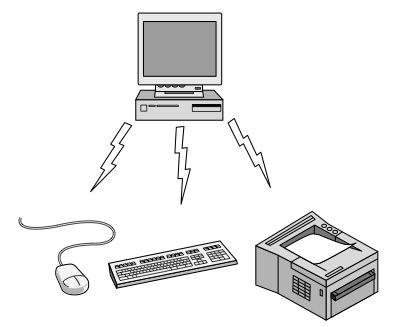
\includegraphics[width=5cm]{figs/05-pan.png}
  \end{center}

\end{frame}

%---------------------------------------------------------------------
\begin{frame}
  \frametitle{LAN: Local Area Network}

  Recursos compartidos a nivel de oficinas o edificios

  \begin{itemize}
    \item Medios basados en cables de cobre o fibra óptica
    \item Tamaño conocido permite acotar tiempos de transmisión
    \item Velocidades: 100Mbps, 1Gbps, 10Gbps
    \item Topología común: punto a punto
    \item Estándar IEEE 802.3: {\bf Ethernet}
    \item {\bf Switch}: dispositivo que dirige paquetes entre dispositivos conectados
    
  \begin{center}
    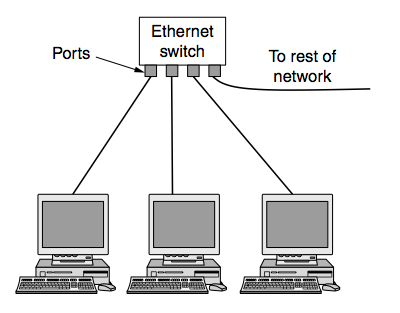
\includegraphics[width=5cm]{figs/05-wiredlan.png}
  \end{center}
    
  \end{itemize}

\end{frame}

%---------------------------------------------------------------------
\begin{frame}
  \frametitle{LAN: Local Area Network}
  \framesubtitle{{\em Ethernet} clásica}
  
  \begin{itemize}
    \item Topología clásica: broadcast
    \item Acceso al medio: ante colisiones cada dispositivo espera un tiempo {\em random}
    \item {\bf Hub}: concentrador. Dispositivo que recibe paquetes y reenvía a todos los dispositivos
          conectados. Topología de bus.
  \end{itemize}
  Es posible subdividir un LAN entre redes más pequeñas
  \begin{itemize}
    \item Tráfico de una LAN puede pasar a otra solamente a través de un punto
    \item {\bf Virtual LAN} o {\bf VLAN}
  \end{itemize}

\end{frame}
%---------------------------------------------------------------------
\begin{frame}
  \frametitle{LAN: Local Area Network}
  \framesubtitle{Wireless LAN}

  {\bf WLAN}
  
  \begin{itemize}
    \item Comunicación vía {\em broadcast}
    \item Comunicación a través de dispositivo: {\bf Access Point}, {\bf Wireless Router}, {\bf Base Station}
    \item Standard de acceso: IEEE 802.11 (WiFi)
    \item Velocidad: desde 6Mbps (802.11a), 54Mbps (802.11g), 150Mbps (802.11n), 866Mbps (802.11ac)
    \item Rango: $\sim 70m$ indoor, $\sim 250m$ outdoor
  \end{itemize}

  \begin{center}
    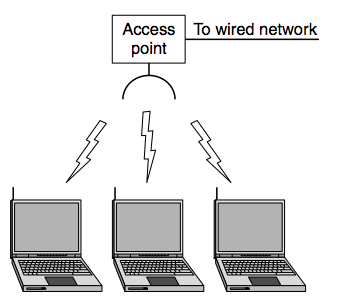
\includegraphics[width=4cm]{figs/05-wirelesslan.png}
  \end{center}

\end{frame}

%---------------------------------------------------------------------
\begin{frame}
  \frametitle{MAN: Metropolitan Area Network}

  \begin{itemize}
    \item Redes de televisión por cable
    \item Standard: IEEE 802.6 DQDB ($\sim 30$km, $34$-$155$Mbps)
    \item Standard: IEEE 802.16 Wireless MAN (WiMax)
    \item Velocidades: $37\sim 219Mbps$ downstream, $17\sim 140Mbps$ upstream
    \item Velocidad límite depende de la distancia (inversamente proporcional)
    \item Rango: kms
  \end{itemize}

  \begin{center}
    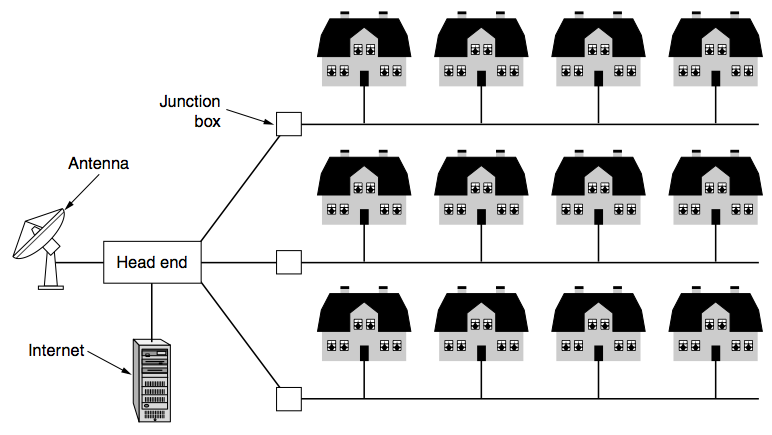
\includegraphics[width=7cm]{figs/05-man.png}
  \end{center}

\end{frame}
%---------------------------------------------------------------------
\begin{frame}
  \frametitle{WAN: Wide Area Network}

  Rango de países o continentes
  \begin{itemize}
    \item Conexión de {\bf hosts} a grandes distancias
    \item Organizada en subredes
  \end{itemize}
  Elementos:
  \begin{itemize}
    \item Líneas de transmisión: cables de cobre, fibra óptica, ondas de radio
    \item {\bf Router}: dispositivo que permite conectar dos o más subredes
    \item Subredes pueden ser redes de diferentes tecnologías
    \item {\em Interredes}: redes compuestas.
      \begin{itemize}
        \item {\bf Internet} es un ejemplo
      \end{itemize}
  \end{itemize}
  Ejemplos wireless:
  \begin{itemize}
    \item Redes satelitales
    \item Redes de celulares (ya en su 4ta generación)
  \end{itemize}
\end{frame}

%---------------------------------------------------------------------
\begin{frame}
  \frametitle{WAN: Wide Area Network}

  Modelo general. Compañía con oficinas en diferentes lugares geográficos
  \begin{center}
    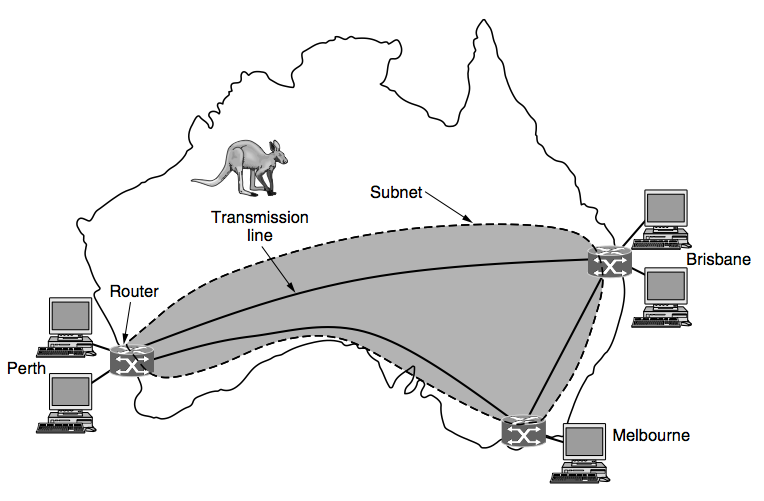
\includegraphics[width=9cm]{figs/05-wan1.png}
  \end{center}

\end{frame}

%---------------------------------------------------------------------
\begin{frame}
  \frametitle{WAN: Wide Area Network}

  {\bf Virtual Private Network} (VPN)
  \begin{itemize}
    \item Formaciones de subredes privadas sobre WAN existentes
    \item Ventaja: virtualización (flexibilidad)
    \item Desventaja: virtualización (calidad de enlace)
  \end{itemize}

  \begin{center}
    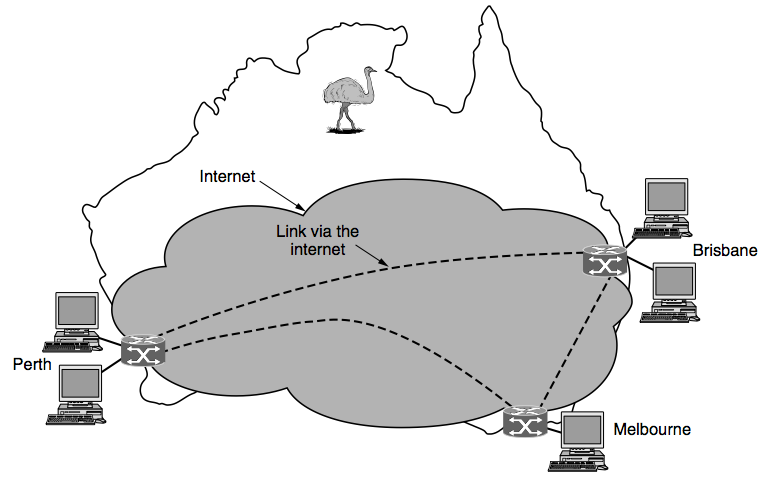
\includegraphics[width=9cm]{figs/05-wan2.png}
  \end{center}

\end{frame}

%---------------------------------------------------------------------
\begin{frame}
  \frametitle{WAN: Wide Area Network}
  
  Subredes operadas por diferentes compañías
  \begin{itemize}
    \item Operador se llama {\bf ISP}: {\bf Internet Service Provider}
    \item Operador permite acceso a su red a clientes
  \end{itemize}
  
  \begin{center}
    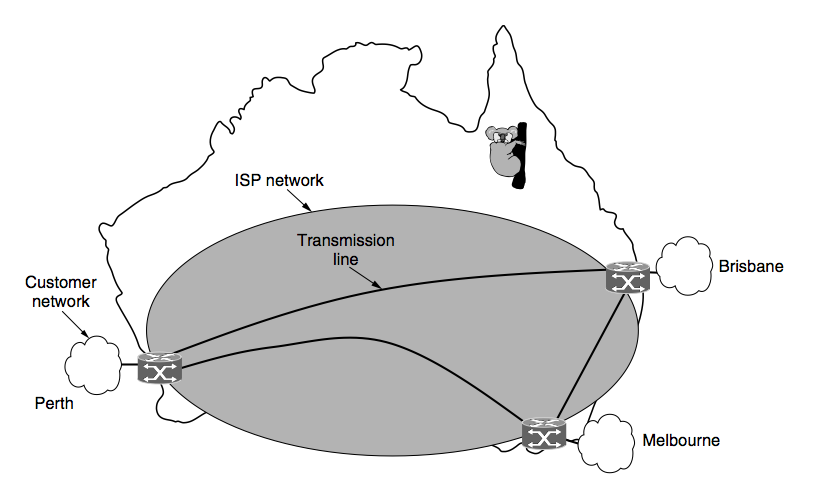
\includegraphics[width=9cm]{figs/05-wan3.png}
  \end{center}

\end{frame}

%---------------------------------------------------------------------
\subsection{Topologías}

\begin{frame}
  \frametitle{Topologías}

  Diferentes topologías para conectar nodos/hosts
  
  \begin{center}
    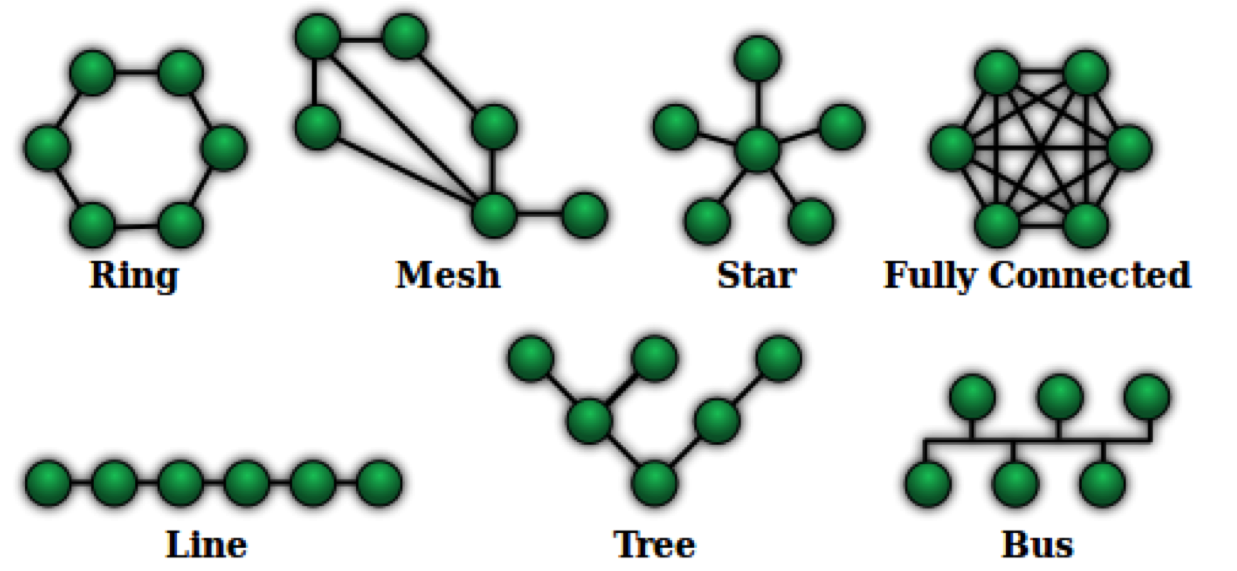
\includegraphics[width=9cm]{figs/05-topologias.png}
  \end{center}
  
\end{frame}

%---------------------------------------------------------------------
\section{Conceptos de {\em Software}}

\subsection{Jerarquías de protocolos}

\begin{frame}
  \frametitle{Jerarquías de protocolos}

  Concepto original: comunicación es problema de {\em hardware}
  \onslide<2->{\ldots {\bf pero ya no}}
   
  \begin{itemize}
    \item<3-> Redes actuales se construyen en capas
    \item<3-> Capas solicitan servicios a niveles inferiores y ofrecen servicios a niveles superiores
    \item<3-> Capas del mismo nivel se comunican a través {\bf protocolos}
  \end{itemize}
  
  \onslide<4->{
  \begin{block}{Protocolo}
    Contrato de comunicación entre distintas partes acerca de la manera
    en que se producirá la comunicación
  \end{block}
  }
\end{frame}

%---------------------------------------------------------------------
\begin{frame}
  \frametitle{Jerarquías de protocolos}

  \begin{center}
    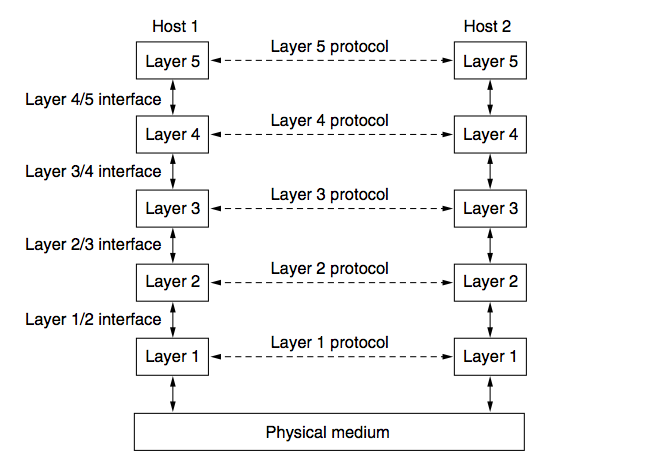
\includegraphics[width=8cm]{figs/05-layers.png}
  \end{center}

  Una instanciación de este modelo se refiere a un {\bf stack de protocolos}
\end{frame}

%---------------------------------------------------------------------
\begin{frame}
  \frametitle{Jerarquías de protocolos}
  
  Mensajes pueden ser modificados en cada capa, agregando {\em headers}
  o modificando todo el mensajes.
  
  \begin{center}
    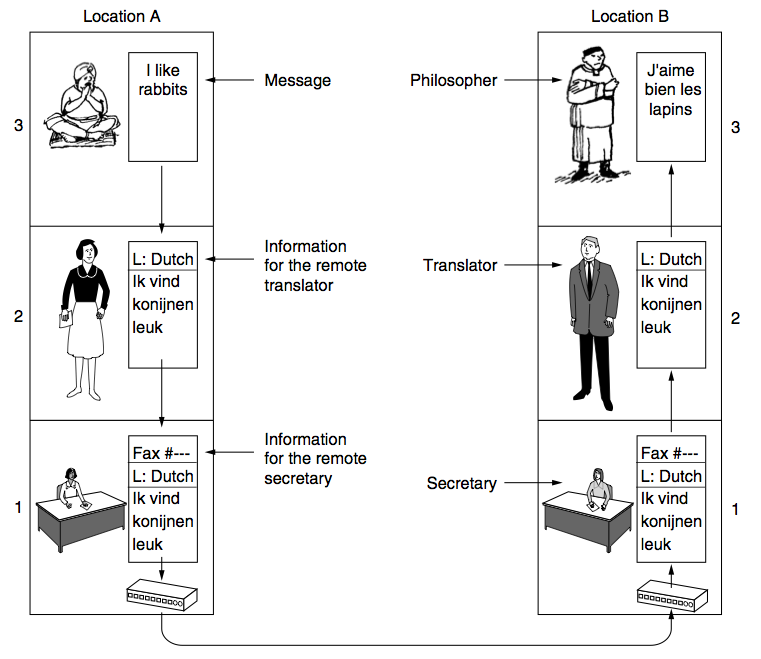
\includegraphics[width=7cm]{figs/05-translations.png}
  \end{center}

\end{frame}
%---------------------------------------------------------------------
\subsection{Servicios y protocolos}

\begin{frame}
  \frametitle{¿Servicios o protocolos?}

  {\bf Servicio}: conjunto de primitivas que ofrecen servicios
  
  {\bf Protocolo}: conjunto de reglas para intercambio y de paquetes y comunicación
  
  \begin{center}
    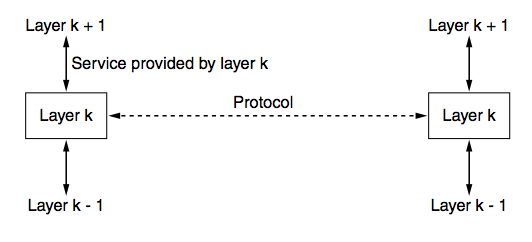
\includegraphics[width=7cm]{figs/05-servicioprotocolo.png}
  \end{center}

  {\bf Importante}: protocolo puede ser cambiado sin afectar al servicio  

\end{frame}
%---------------------------------------------------------------------
\begin{frame}
  \frametitle{Un servicio de comunicación}
  
  Servicio de comunicación basado en Berkeley Sockets
  
  \begin{itemize}
    \item {\tt LISTEN}: bloquea esperando conexión
    \item {\tt CONNECT}: establece conexión con un {\em peer}
    \item {\tt ACCEPT}: acepta conexión desde un {\em peer}
    \item {\tt RECEIVE}: bloquea esperando un mensaje
    \item {\tt SEND}: envía un mensaje al {\em peer}
    \item {\tt DISCONNECT}: cierra conexión
  \end{itemize}
  
\end{frame}

%---------------------------------------------------------------------
\begin{frame}
  \frametitle{Un protocolo de comunicación}

  Protocolo de comunicación
  \begin{itemize}
    \item Server ejecuta {\tt LISTEN}
    \item Client ejecuta {\tt CONNECT} especificando dirección del servidor
      \begin{itemize}
        \item SO envía paquete y bloquea al client esperando respuesta
      \end{itemize}
    \item SO recibe paquete, busca algún proceso que haya hecho {\tt LISTEN}, copia paquete y desbloquea
    \item Server puede decidir si acepta la conexión haciendo {\tt ACCEPT}
      \begin{itemize}
        \item SO server envía mensajes de aceptación a client
        \item SO client recibe mensaje y desbloquea a proceso client
      \end{itemize}
    \item Proceso client y server quedan conectados y puede enviarse mensajes
  \end{itemize}
\end{frame}

%---------------------------------------------------------------------
\begin{frame}
  \frametitle{Un protocolo de comunicación}

  \begin{itemize}
    \item Server ejecuta {\tt RECEIVE} para esperar mensajes
    \item Client ejecuta {\tt SEND} para enviar mensajes
    \item Client finaliza comunicación con {\tt DISCONNECT}
  \end{itemize}
  
  \begin{center}
    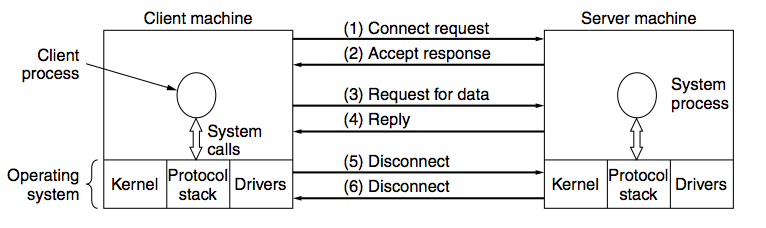
\includegraphics[width=10cm]{figs/05-ejemploprotocolo.png}
  \end{center}

  Por supuesto, éste es el {\em happy-path}

\end{frame}
%---------------------------------------------------------------------
\section{Modelos de referencia}

\subsection{Modelo OSI}

\begin{frame}
  \frametitle{Modelo OSI}

  Estándar ISO {\bf OSI} ({\bf Open Systems Interface})
  \begin{itemize}
    \item Propuesto en 1983 por Day y Zimmerman
    \item Revisado en 1995
    \item Es un {\bf modelo de referencia}
      \begin{itemize}
        \item Define responsabilidades para cada capa
        \item No define estándares ni protocolos
        \item No establece implementaciones
      \end{itemize}
  \end{itemize}
  
\end{frame}
%---------------------------------------------------------------------
\begin{frame}
  \frametitle{Modelo OSI}
  \framesubtitle{Oh, sí, oh, sí}

  \begin{center}
    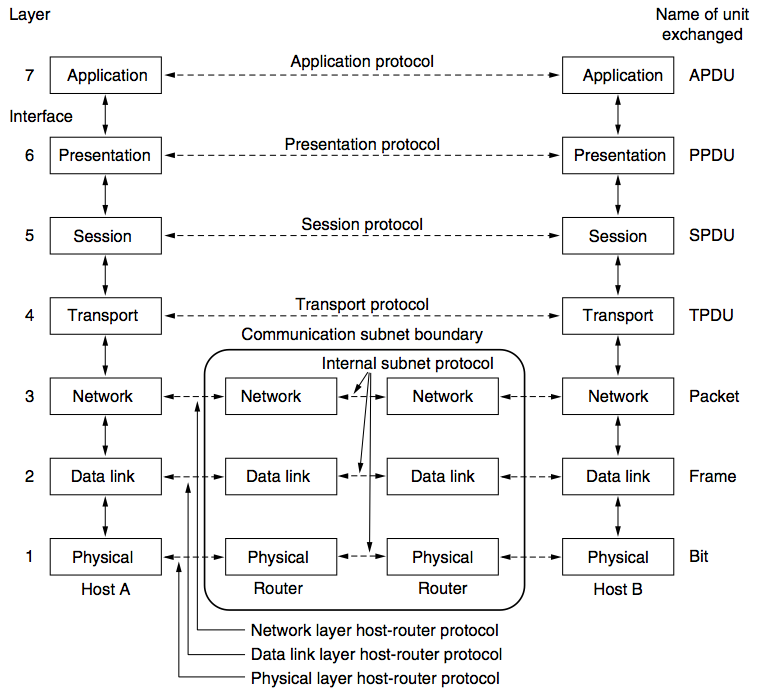
\includegraphics[width=8cm]{figs/05-osi.png}
  \end{center}
  
\end{frame}

%---------------------------------------------------------------------
\begin{frame}
  \frametitle{Modelo OSI}
  \framesubtitle{¿Qué hace cada nivel?}

  \begin{itemize}
    \item {\bf Capa Física}. Transmisión de {\bf bits} en canal de comunicación.
      \begin{itemize}
        \item Tiempo de transmisión, frecuencia de transmisición, codificación
      \end{itemize}
    \item {\bf Capa de Enlace} ({\em data link}). Transmisión secuencial de grupos de bits: {\bf frames}
          de manera que lleguen sin errores.
      \begin{itemize}
        \item Control de velocidad de transmisión.
        \item Control de acceso al medio (MAC)
      \end{itemize}
    \item {\bf Capa de Red} ({\em network}). Transmisión de paquetes de datos entre nodos de la red.
      \begin{itemize}
        \item ¿Cómo encontrar al destinatario? Direccionamiento
        \item ¿Qué ruta deben seguir los paquetes para llegar?
      \end{itemize}
  \end{itemize}
\end{frame}

%---------------------------------------------------------------------
\begin{frame}
  \frametitle{Modelo OSI}
  \framesubtitle{¿Qué hace cada nivel?}

  \begin{itemize}
    \item {\bf Capa de Transporte}. Transmisión del mensajes solicitados desde la fuentel espacio al destinatario
      \begin{itemize}
        \item Orden y velocidad de transmisión de paquetes (control de flujo)
        \item ¿Cómo asegurar que todos los paquetes hayan llegado?
        \item Connection-oriented vs connection-less
      \end{itemize}
    \item {\bf Capa de Sesión}. Mantenimiento de sesiones, turnos de transmisión, sincronización
    \item {\bf Capa de Presentación}. Definición de sintaxis y semántica de datos a transmitir.
    \item {\bf Capa de Aplicación}. Protocolos de comunicación entre procesos para objetivos específicos
      \begin{itemize}
        \item HTTP, FTP, SSH, SMTP, IMAP, XMPP, DNS, TELNET, DHCP, \ldots
      \end{itemize}
  \end{itemize}
\end{frame}

%---------------------------------------------------------------------
\subsection{Modelo TCP/IP}

\begin{frame}
  \frametitle{Modelo TCP/IP}

  Originado como {\em stack} de protocolos para ARPANET, proyecto de investigación del DoD (Department of Defense, USA)
  \begin{itemize}
    \item Propuesto por Vinton Cerf y Robert E. Kahn, 1974
    \item Estandarizado en 1989
  \end{itemize}

  \begin{center}
    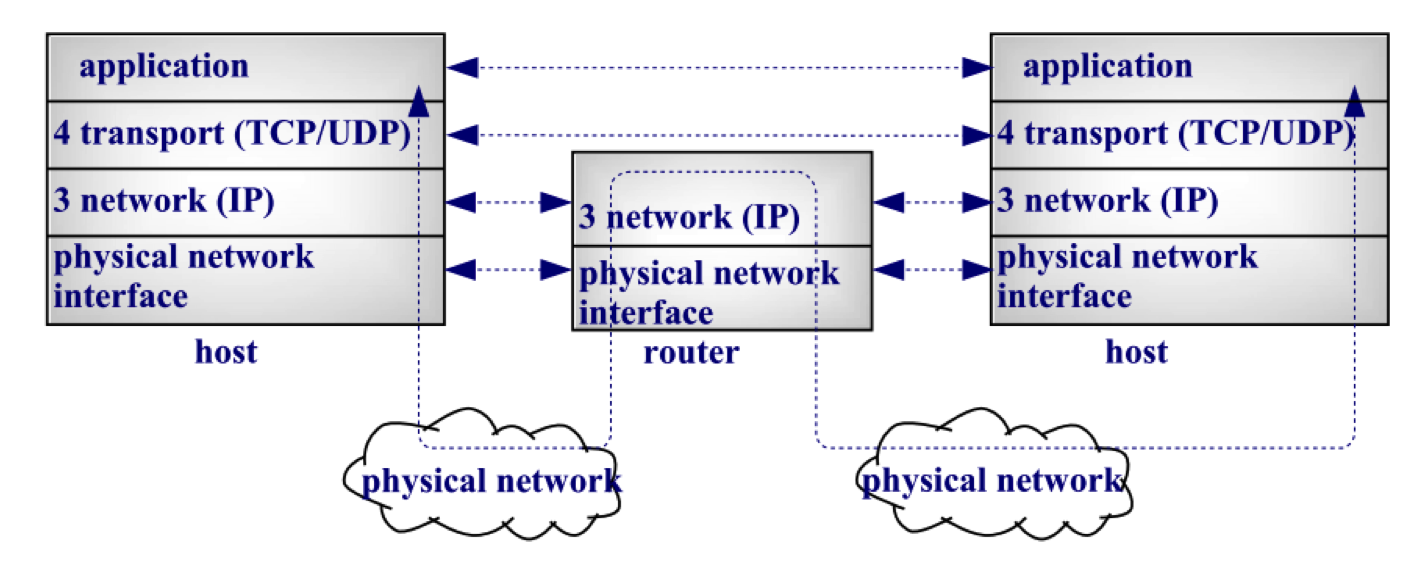
\includegraphics[width=10cm]{figs/05-tcpip.png}
  \end{center}

\end{frame}
%---------------------------------------------------------------------
\begin{frame}
  \frametitle{Modelo TCP/IP}

  \begin{itemize}
    \item {\bf Link layer}. Incluye funciones de capas OSI 1 y 2.
      \begin{itemize}
        \item Inyección de paquetes de capa superior a algún medio de transmisión .
        \item También llamado {\em host-to-network}. Poco especificada.
      \end{itemize}
    \item {\bf Internet layer} (interred). Transmisión de paquetes entre redes.
      \begin{itemize}
        \item Protocolo IP. Internet Protocol.
        \item Protocolo ICMP. Internet Control Message Protocol.
      \end{itemize}
    \item {\bf Transport layer}. Transmisión de mensajes entre fuente y destinatario.
      \begin{itemize}
        \item TCP. Transmission Control Protocol. Connection-oriented.
        \item UDP. User Datagram Protocol. Connectionless.
      \end{itemize}
    \item {\bf Application Layer}. Equivalente a capas 5,6 y 7 de OSI.
      \begin{itemize}
        \item Protocolos de aplicaciones visibles para el usuario.
        \item Conexiones a través de {\em sockets}.
        \item Servicios estandarizados en {\em well-known} ports por {\bf IANA} (Internet Assigned Numbers Authority)
      \end{itemize}
  \end{itemize}
\end{frame}
%---------------------------------------------------------------------
\begin{frame}
  \frametitle{Modelo TCP/IP}

  \begin{center}
    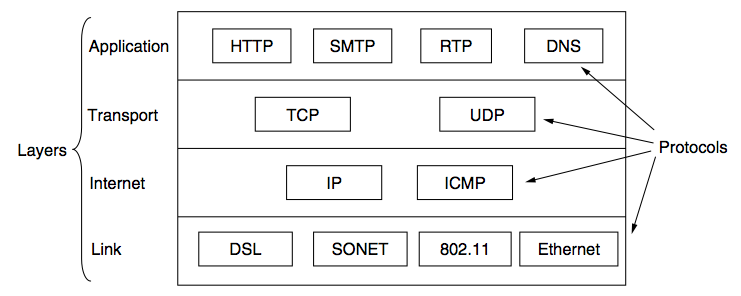
\includegraphics[width=10cm]{figs/05-protocolstcpip.png}
  \end{center}

\end{frame}
%---------------------------------------------------------------------
\begin{frame}
  \frametitle{Mensajes}

  Mensajes van adquiriendo {\em header}s en cada capa
  
  \begin{center}
    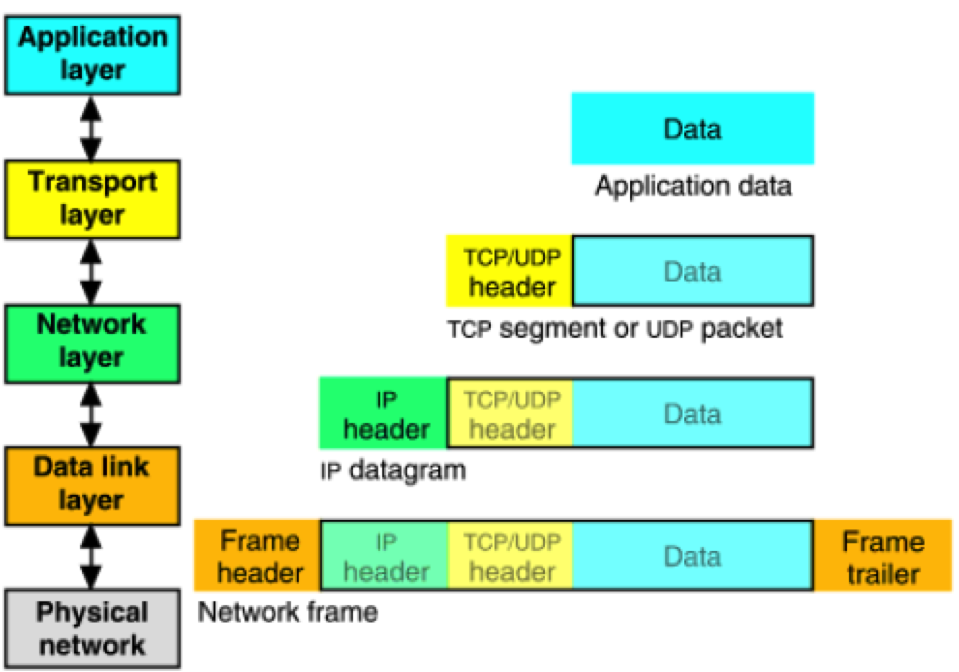
\includegraphics[width=9cm]{figs/05-mensajes.png}
  \end{center}

\end{frame}

%---------------------------------------------------------------------
\begin{frame}
  \frametitle{Mensajes}

  {\em Header} TCP

  \begin{center}
    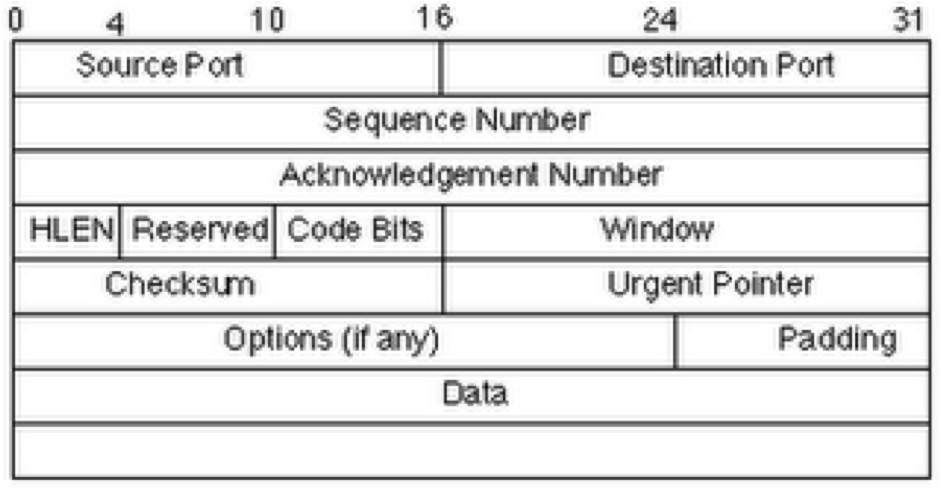
\includegraphics[width=8cm]{figs/05-headertcp.png}
  \end{center}

\end{frame}
%---------------------------------------------------------------------
\begin{frame}
  \frametitle{Mensajes}

  {\em Header} IP
  
  \begin{center}
    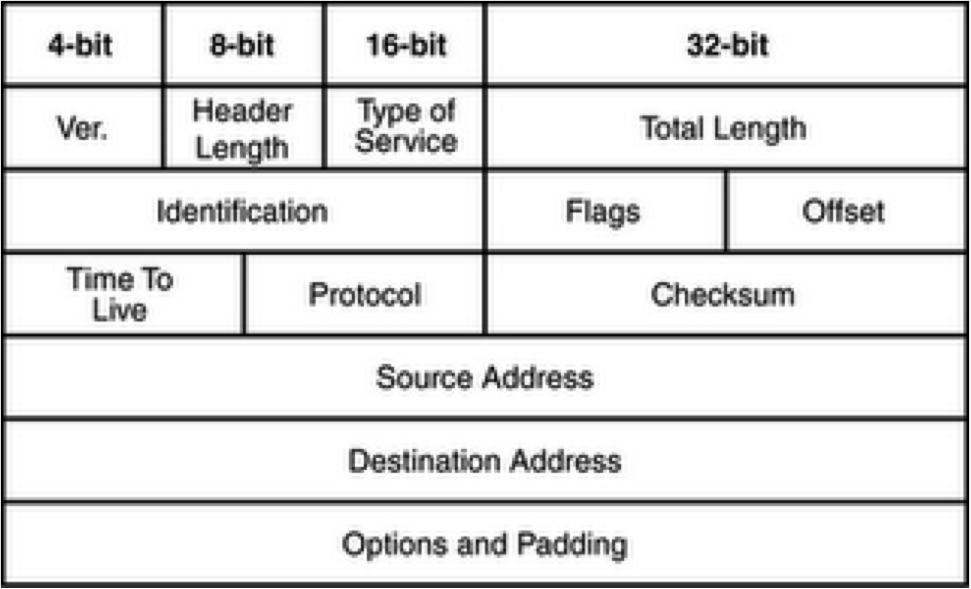
\includegraphics[width=8cm]{figs/05-headerip.png}
  \end{center}
  

\end{frame}
%---------------------------------------------------------------------
\begin{frame}
  \frametitle{Mensajes}

  Paquete 802.11

  \begin{center}
    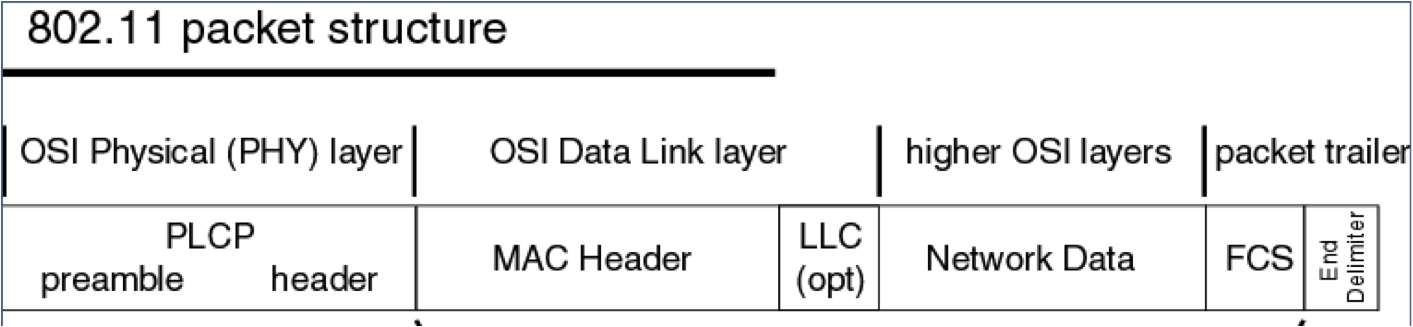
\includegraphics[width=10cm]{figs/05-header80211.png}
  \end{center}
  
  

\end{frame}
%---------------------------------------------------------------------
\begin{frame}
  \frametitle{Redes: Internet}

  \begin{center}
    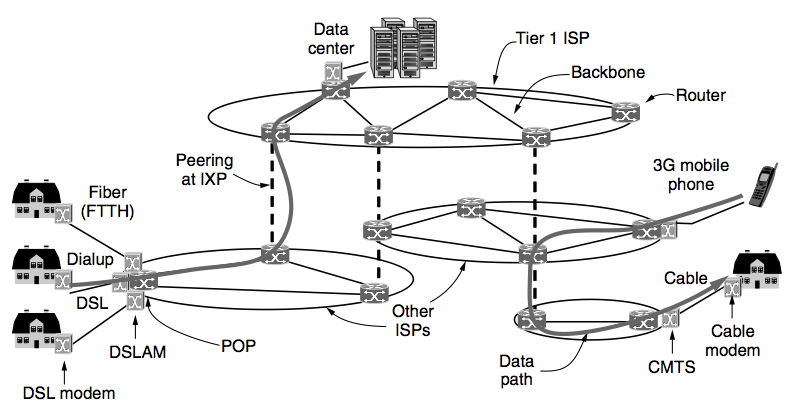
\includegraphics[width=11cm]{figs/05-internet.png}
  \end{center}

\end{frame}

%---------------------------------------------------------------------
\begin{frame}
  \frametitle{Redes: Internet}

  \url{http://www.submarinecablemap.com/}

\end{frame}

%---------------------------------------------------------------------
\begin{frame}
  \frametitle{Redes: Telefonía Móvil}

  \begin{itemize}
    \item 1G. AMPS (Advanced Mobile Phone System). Análogo, 1982.
    \item 2G. GSM (Global System for Mobile Communications) 1991.
    \item 3G. Voz digital + banda ancha de datos, 2001.
      \begin{itemize}
        \item UMTS (Universal Mobile Telecommunications Systems)
              a.k.a. WCDMA (Wideband Code Division Multiple Access)
        \item $\sim 14$Mbps {\em downlink}, $\sim 6$Mbps {\em uplink}
        \item Recurso escaso: espectro de frecuencias
        \item Celdas adyacentes usan frecuencias distintas
      \end{itemize}
  \end{itemize}
  
  \begin{center}
    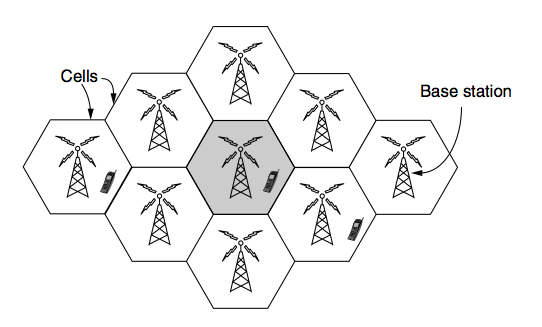
\includegraphics[width=8cm]{figs/05-mobile1.png}
  \end{center}

\end{frame}

%---------------------------------------------------------------------
\begin{frame}
  \frametitle{Redes: Telefonía Móvil}

  Arquitectura
  \begin{itemize}
    \item RNC, Radio Network Controller
    \item PSTN, Public Switched Telephone Network
  \end{itemize}
  \begin{center}
    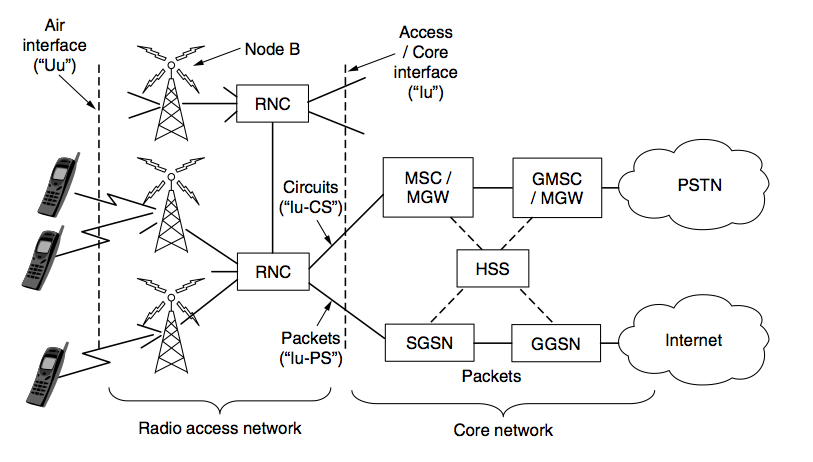
\includegraphics[width=10cm]{figs/05-mobile2.png}
  \end{center}

\end{frame}

%---------------------------------------------------------------------
\begin{frame}
  \frametitle{Redes: Telefonía Móvil}
  \framesubtitle{Handover $\neq$ hangover}

  Redes móviles tienen el desafío del {\bf handover}
  \begin{itemize}
    \item {\bf Hard handover}. Desconectarse de una celda antes de conectarse a la siguiente.
    \item {\bf Soft handover}. Mantener la conexión hasta encontrar otra celda.
  \end{itemize}
  \begin{center}
    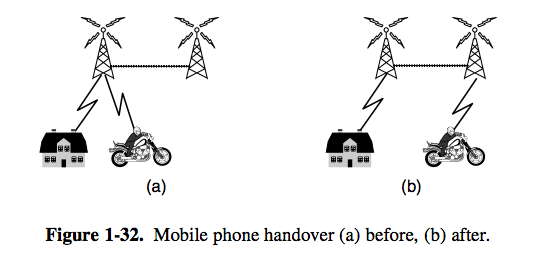
\includegraphics[width=10cm]{figs/05-mobile3.png}
  \end{center}

\end{frame}
%---------------------------------------------------------------------
\end{document}